%%%%%%%%%%%%%%%%%%%%%%%%%%%%%%%%%%%%%%%%%
% Beamer Presentation
% LaTeX Template
% Version 1.0 (10/11/12)
%
% This template has been downloaded from:
% http://www.LaTeXTemplates.com
%
% License:
% CC BY-NC-SA 3.0 (http://creativecommons.org/licenses/by-nc-sa/3.0/)
%
%%%%%%%%%%%%%%%%%%%%%%%%%%%%%%%%%%%%%%%%%

%----------------------------------------------------------------------------------------
%	PACKAGES AND THEMES
%----------------------------------------------------------------------------------------

\documentclass{beamer}
\usepackage[utf8]{inputenc}
\usepackage[T1]{fontenc}
\usepackage[brazil]{babel}
\usepackage{amsmath}
\usepackage{amsfonts}
\usepackage{amssymb}
\mode<presentation> {

% The Beamer class comes with a number of default slide themes
% which change the colors and layouts of slides. Below this is a list
% of all the themes, uncomment each in turn to see what they look like.

%\usetheme{default}
%\usetheme{AnnArbor}
%\usetheme{Antibes}
%\usetheme{Bergen}
%\usetheme{Berkeley}
%\usetheme{Berlin}
%\usetheme{Boadilla}
\usetheme{CambridgeUS}
%\usetheme{Copenhagen}
%\usetheme{Darmstadt}
%\usetheme{Dresden}
%\usetheme{Frankfurt}
%\usetheme{Goettingen}
%\usetheme{Hannover}
%\usetheme{Ilmenau}
%\usetheme{JuanLesPins}
%\usetheme{Luebeck}
%\usetheme{Madrid}
%\usetheme{Malmoe}
%\usetheme{Marburg}
%\usetheme{Montpellier}
%\usetheme{PaloAlto}
%\usetheme{Pittsburgh}
%\usetheme{Rochester}
%\usetheme{Singapore}
%\usetheme{Szeged}
%\usetheme{Warsaw}

% As well as themes, the Beamer class has a number of color themes
% for any slide theme. Uncomment each of these in turn to see how it
% changes the colors of your current slide theme.

%\usecolortheme{albatross}
%\usecolortheme{beaver}
%\usecolortheme{beetle}
%\usecolortheme{crane}
%\usecolortheme{dolphin}
%\usecolortheme{dove}
%\usecolortheme{fly}
%\usecolortheme{lily}
%\usecolortheme{orchid}
%\usecolortheme{rose}
%\usecolortheme{seagull}
%\usecolortheme{seahorse}
%\usecolortheme{whale}
%\usecolortheme{wolverine}

%\setbeamertemplate{footline} % To remove the footer line in all slides uncomment this line
%\setbeamertemplate{footline}[page number] % To replace the footer line in all slides with a simple slide count uncomment this line

%\setbeamertemplate{navigation symbols}{} % To remove the navigation symbols from the bottom of all slides uncomment this line
}

\usepackage{graphicx} % Allows including images
\usepackage{booktabs} % Allows the use of \toprule, \midrule and \bottomrule in tables

%----------------------------------------------------------------------------------------
%	TITLE PAGE
%----------------------------------------------------------------------------------------

\title[ENAPOL 2018 ]{Representando Significado com Vetores} % The short title appears at the bottom of every slide, the full title is only on the title page

\author{Bruno Ferrari Guide} % Your name
\institute[USP] % Your institution as it will appear on the bottom of every slide, may be shorthand to save space
{Orientador: Marcos Lopes\\
Universidade de São Paulo \\ % Your institution for the title page
\medskip
\textit{bruno.guide@usp.br} % Your email address
}
\date{\today} % Date, can be changed to a custom date

\begin{document}

\begin{frame}
\titlepage % Print the title page as the first slide
\end{frame}

\begin{frame}
\frametitle{Tópicos} % Table of contents slide, comment this block out to remove it
\tableofcontents % Throughout your presentation, if you choose to use \section{} and \subsection{} commands, these will automatically be printed on this slide as an overview of your presentation
\end{frame}

%----------------------------------------------------------------------------------------
%	PRESENTATION SLIDES
%----------------------------------------------------------------------------------------

%------------------------------------------------
\section{Vetorizando a Língua} % Sections can be created in order to organize your presentation into discrete blocks, all sections and subsections are automatically printed in the table of contents as an overview of the talk
%------------------------------------------------


\begin{frame}
\begin{itemize}
    \item \Large{Vetorizando a Língua}

\end{itemize}

\end{frame}

%------------------------------------------------

\begin{frame}
\frametitle{Juntando e contando coisas - Corpora e estatística}
\begin{figure}
	\centering
	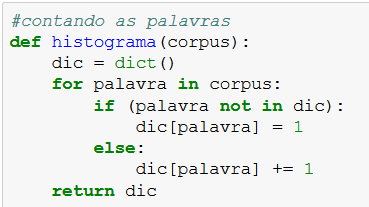
\includegraphics[width=0.7\linewidth]{Contando}
	\caption{Script em Python para contar palavras}
	\label{fig:contando}
\end{figure}

\end{frame}

%------------------------------------------------



\begin{frame}
\frametitle{Frequência de termo (TF)}
\begin{figure}
	\centering
	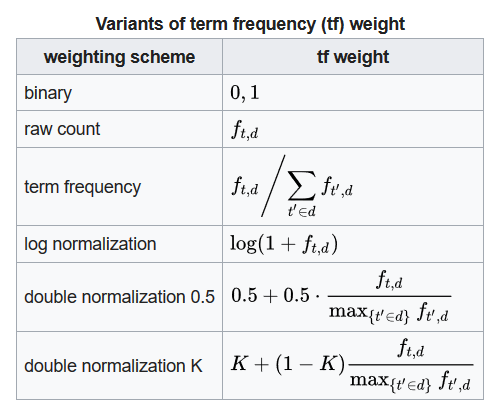
\includegraphics[width=0.7\linewidth]{TF}
	%\caption{}
	\label{fig:tf}
\end{figure}
\end{frame}


%------------------------------------------------

\begin{frame}
\frametitle{Matriz de termos-documentos}
\begin{figure}
	\centering
	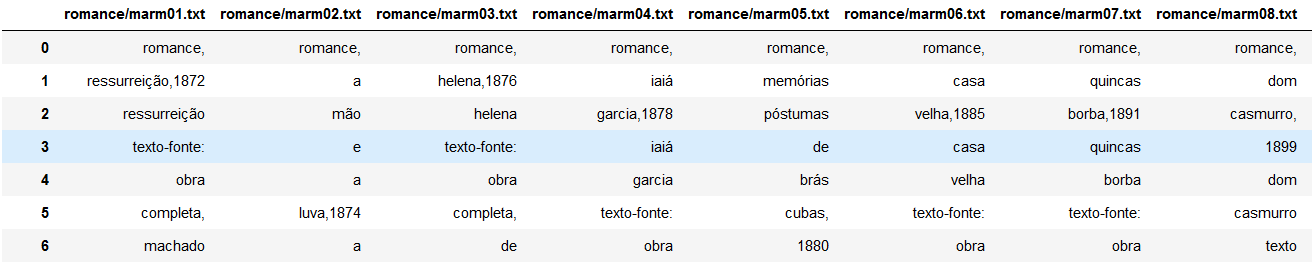
\includegraphics[width=0.7\linewidth]{matriz}
	\caption{Matriz termo-documento}
	\label{fig:matriz}
\end{figure}

\end{frame}

%------------------------------------------------

\begin{frame}
\frametitle{Frequência inversa em documentos (IDF)}
\begin{figure}
	\centering
	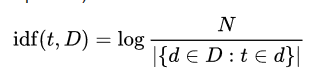
\includegraphics[width=0.7\linewidth]{idf}
	\caption{Inverse Document Frequency}
	\label{fig:idf}
\end{figure}
	
\end{frame}

%------------------------------------------------

\begin{frame}
\frametitle{TF-IDF}
\begin{figure}
	\centering
	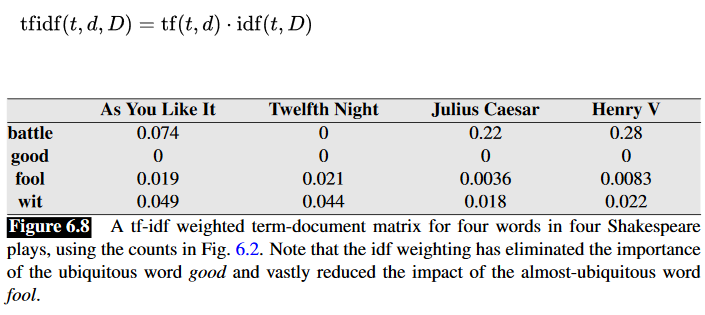
\includegraphics[width=0.7\linewidth]{tf-idf(short)}
	\caption{TF-IDF com exemplo}
	\label{fig:tf-idfshort}
\end{figure}

\end{frame}

%------------------------------------------------


%------------------------------------------------
\section{Um breve desvio: Vetores, Álgebra e Geometria}
%------------------------------------------------

\begin{frame}
\begin{itemize}
    \item \Large{Vetores, Álgebra e Geometria}

\end{itemize}

\end{frame}
%------------------------------------------------

\begin{frame}
\frametitle{Plano Cartesiano}

\begin{figure}
	\centering
	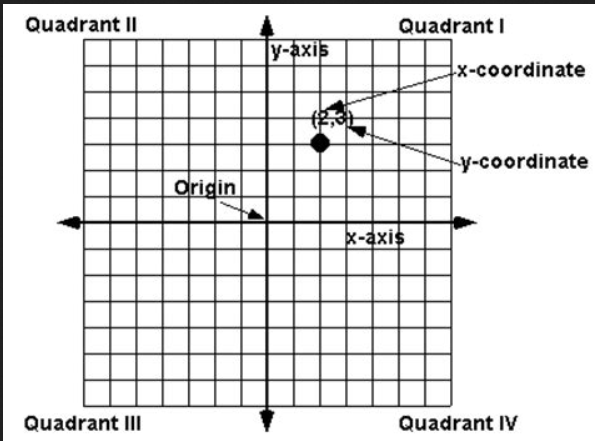
\includegraphics[width=0.7\linewidth]{descartes1}
	\caption[]{O plano Cartesiano}
	\label{fig:descartes1}
\end{figure}
\end{frame}

%------------------------------------------------

\begin{frame}
\frametitle{Ponto e vetor}
\begin{figure}
	\centering
	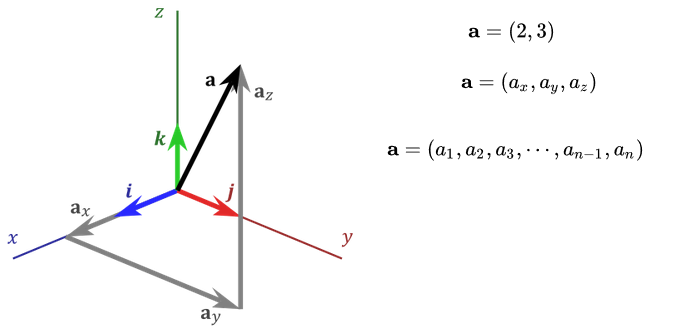
\includegraphics[width=0.7\linewidth]{vector_dimensions}
	\caption[]{Pontos, Vetores e dimensões}
	\label{fig:vectordimensions}
\end{figure}

\end{frame}

%------------------------------------------------

\begin{frame}
\frametitle{Palavras são vetores}
\begin{figure}
	\centering
	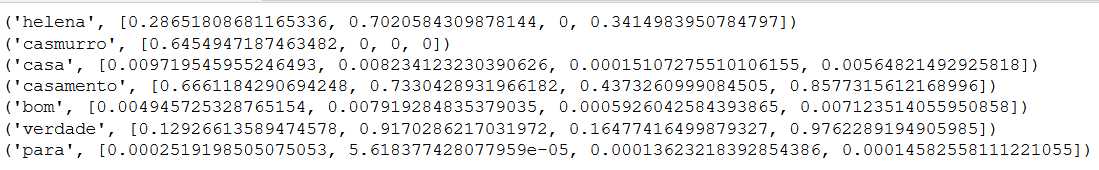
\includegraphics[width=0.7\linewidth]{word_vectors}
	\caption{Vetores de palavras}
	\label{fig:wordvectors}
\end{figure}

\end{frame}

%------------------------------------------------

\begin{frame}
\frametitle{Distância entre vetores}
\begin{figure}
	\centering
	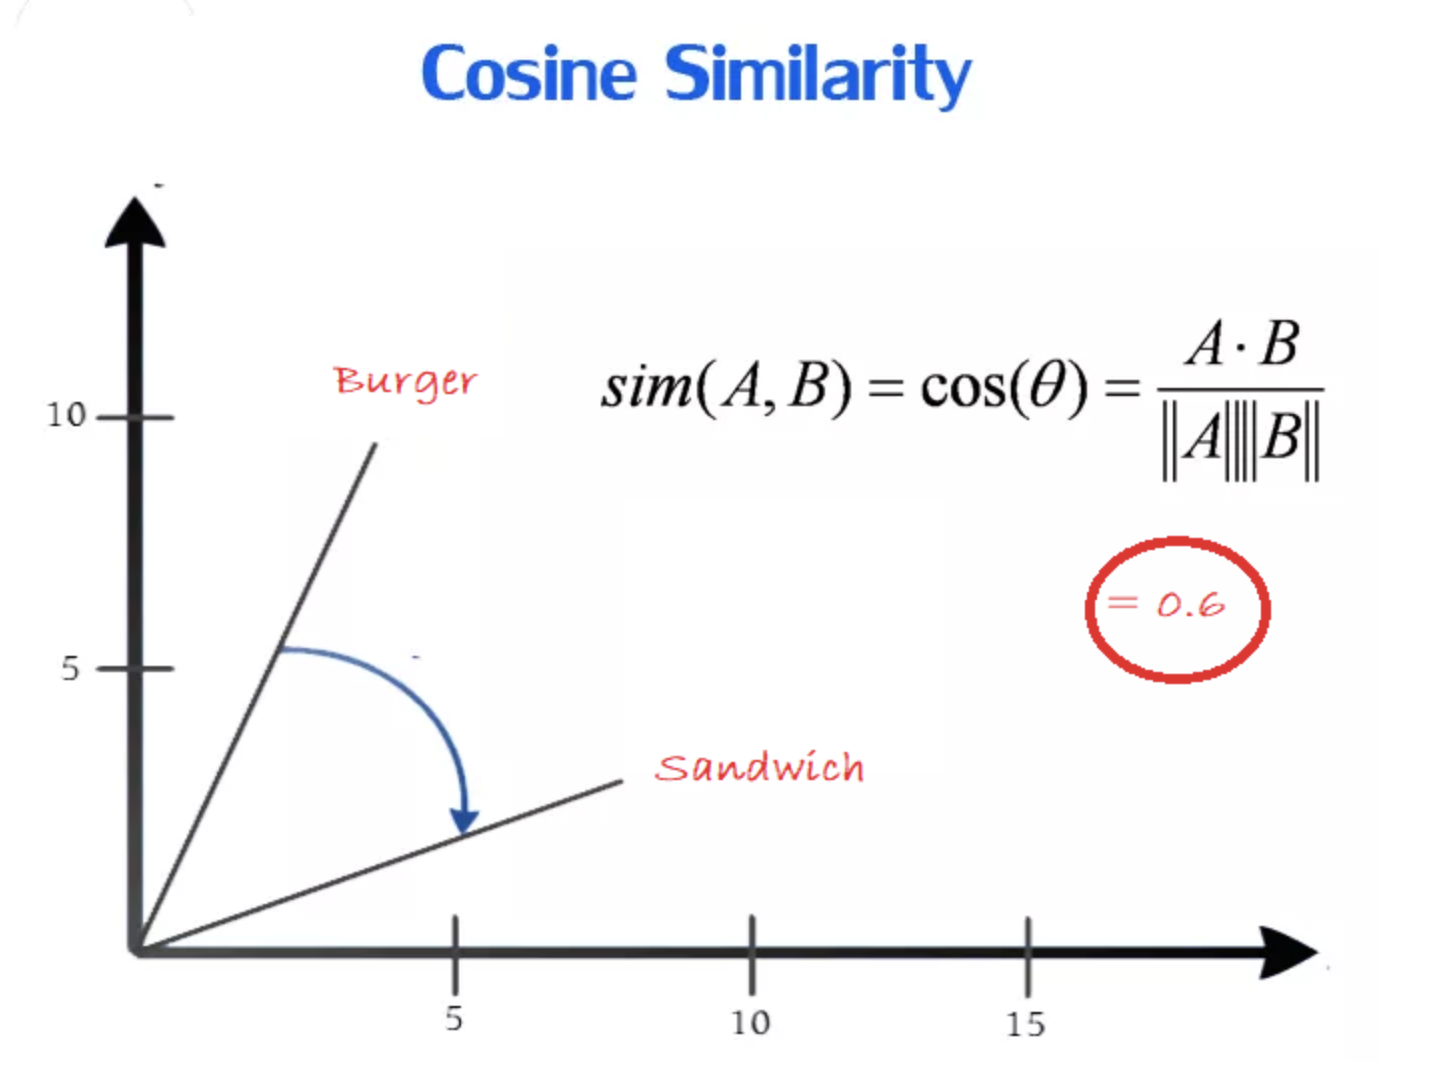
\includegraphics[width=0.7\linewidth]{cosine_sim}
	\caption{Similaridade de cosseno}
	\label{fig:cosinesim}
\end{figure}

\end{frame}


%------------------------------------------------

%------------------------------------------------
\section{Vetores Esparsos e Densos}
%------------------------------------------------

\begin{frame}
\begin{itemize}
    \item \Large{Vetores Esparsos e Densos}

\end{itemize}

\end{frame}
%------------------------------------------------

\begin{frame}
\frametitle{A Maldição da Dimensionalidade}
\begin{figure}
	\centering
	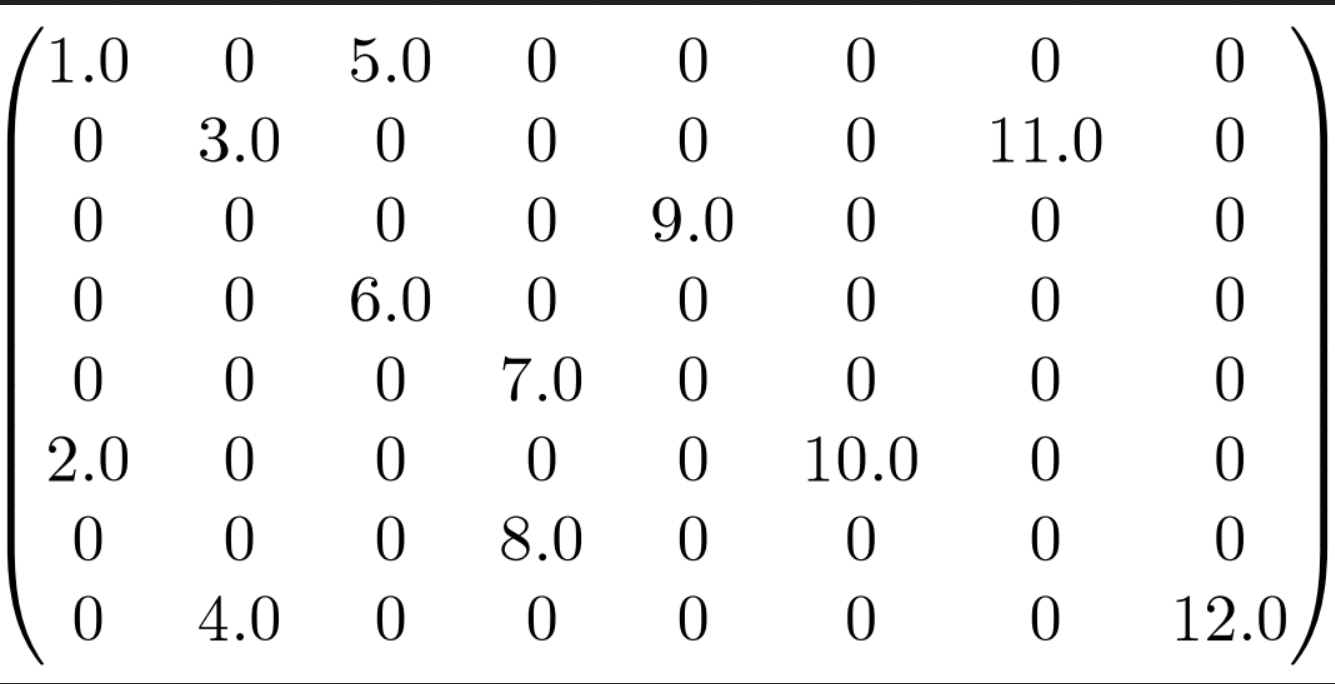
\includegraphics[width=0.7\linewidth]{spM}
	\caption{Coleção de Vetores (Matriz)}
	\label{fig:spm}
\end{figure}

\end{frame}

%------------------------------------------------

\begin{frame}
\frametitle{Vetores Densos vs. Vetores Esparsos}
\begin{table}
	\begin{tabular}{l l l}
		\toprule
		\textbf{Tipo de Vetor} & \textbf{Interpretação} & \textbf{Exigência para processamento}\\
		\midrule
		Esparso & Transparente & Exigente \\
		Denso & Opaco & Amigável \\
		\bottomrule
	\end{tabular}
	\caption{Comparação entre vetores densos e esparsos}
\end{table}
\end{frame}

%------------------------------------------------

%------------------------------------------------

%------------------------------------------------

\begin{frame}
\frametitle{Adensando Vetores}
\begin{figure}
	\centering
	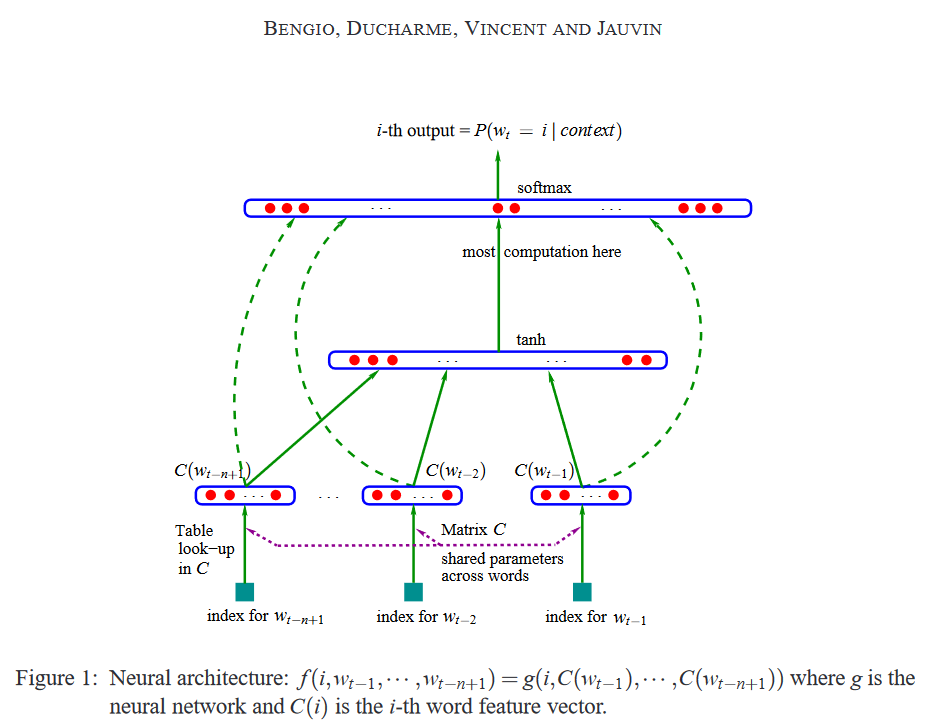
\includegraphics[width=0.7\linewidth]{bengio03}
	\caption{É possível, mas não cabe a discussão no momento}
	\label{fig:bengio03}
\end{figure}

\end{frame}

%------------------------------------------------

\begin{frame}
\frametitle{Funciona?}
\begin{itemize}
\item Muito!\\
\item Hoje a semântica de vetores densos é dominante nos algoritmos mais bem sucedidos para interpretação de significado, como chatbots, tradução automática, busca.\\
\item Os modelos principais não são iguais a LSA do slide anterior, mas o principio de adensar vetores é o mesmo.\\
\item A seguir, explorarei os tipos de relação semântica que podemos explorar nos vetores gerados pelo modelo Word2Vec.\\
\end{itemize}
\end{frame}

%------------------------------------------------



%------------------------------------------------
\section{Noções Linguísticas Subjacentes}
%------------------------------------------------

\begin{frame}
\begin{itemize}
    \item \Large{Noções Linguísticas Subjacentes}

\end{itemize}

\end{frame}
%------------------------------------------------

\begin{frame}
\frametitle{Operações com vetores - similaridade}
\begin{figure}
	\centering
	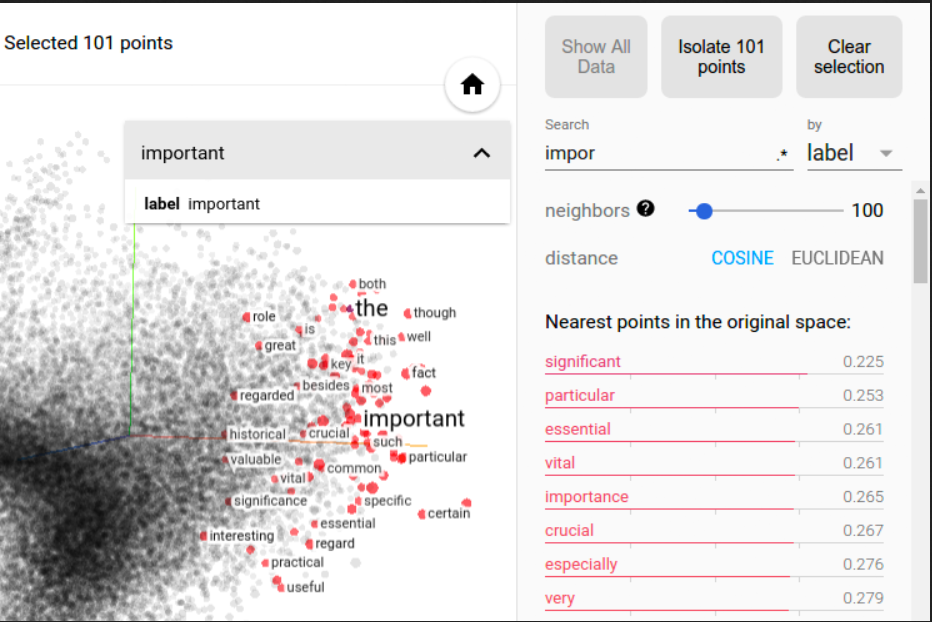
\includegraphics[width=0.7\linewidth]{w2v-tensorflow}
	\caption{Similaridade com Word2Vec}
	\label{fig:w2v-tensorflow}
\end{figure}

\end{frame}

%------------------------------------------------

\begin{frame}
\frametitle{Operações com vetores - linearidades}
\begin{figure}
	\centering
	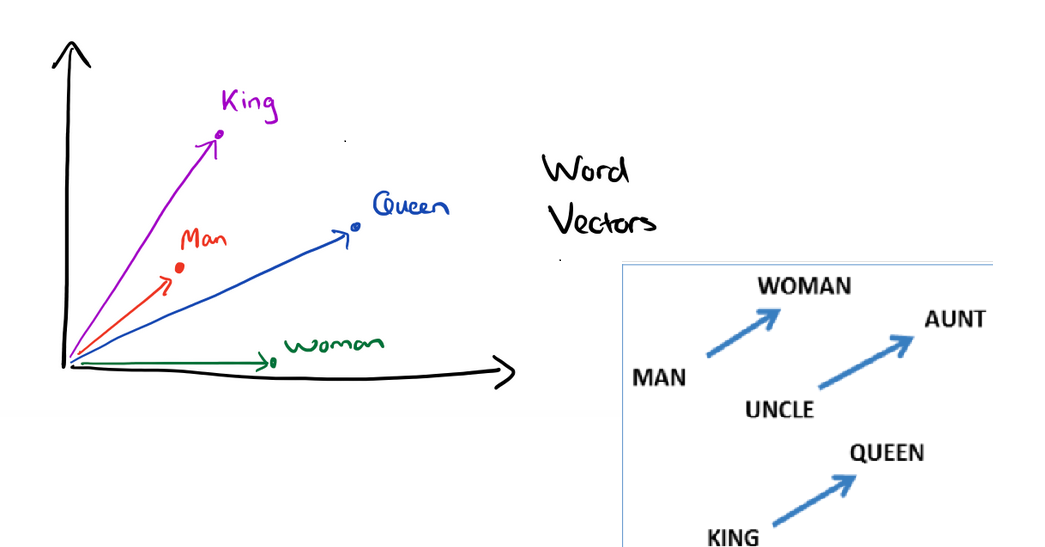
\includegraphics[width=0.7\linewidth]{linearidades-2}
	\caption{Relações lineares}
	\label{fig:linearidades-2}
\end{figure}

\end{frame}

%------------------------------------------------
\begin{frame}
\frametitle{ O que um vetor codifica?}
\begin{figure}
	\centering
	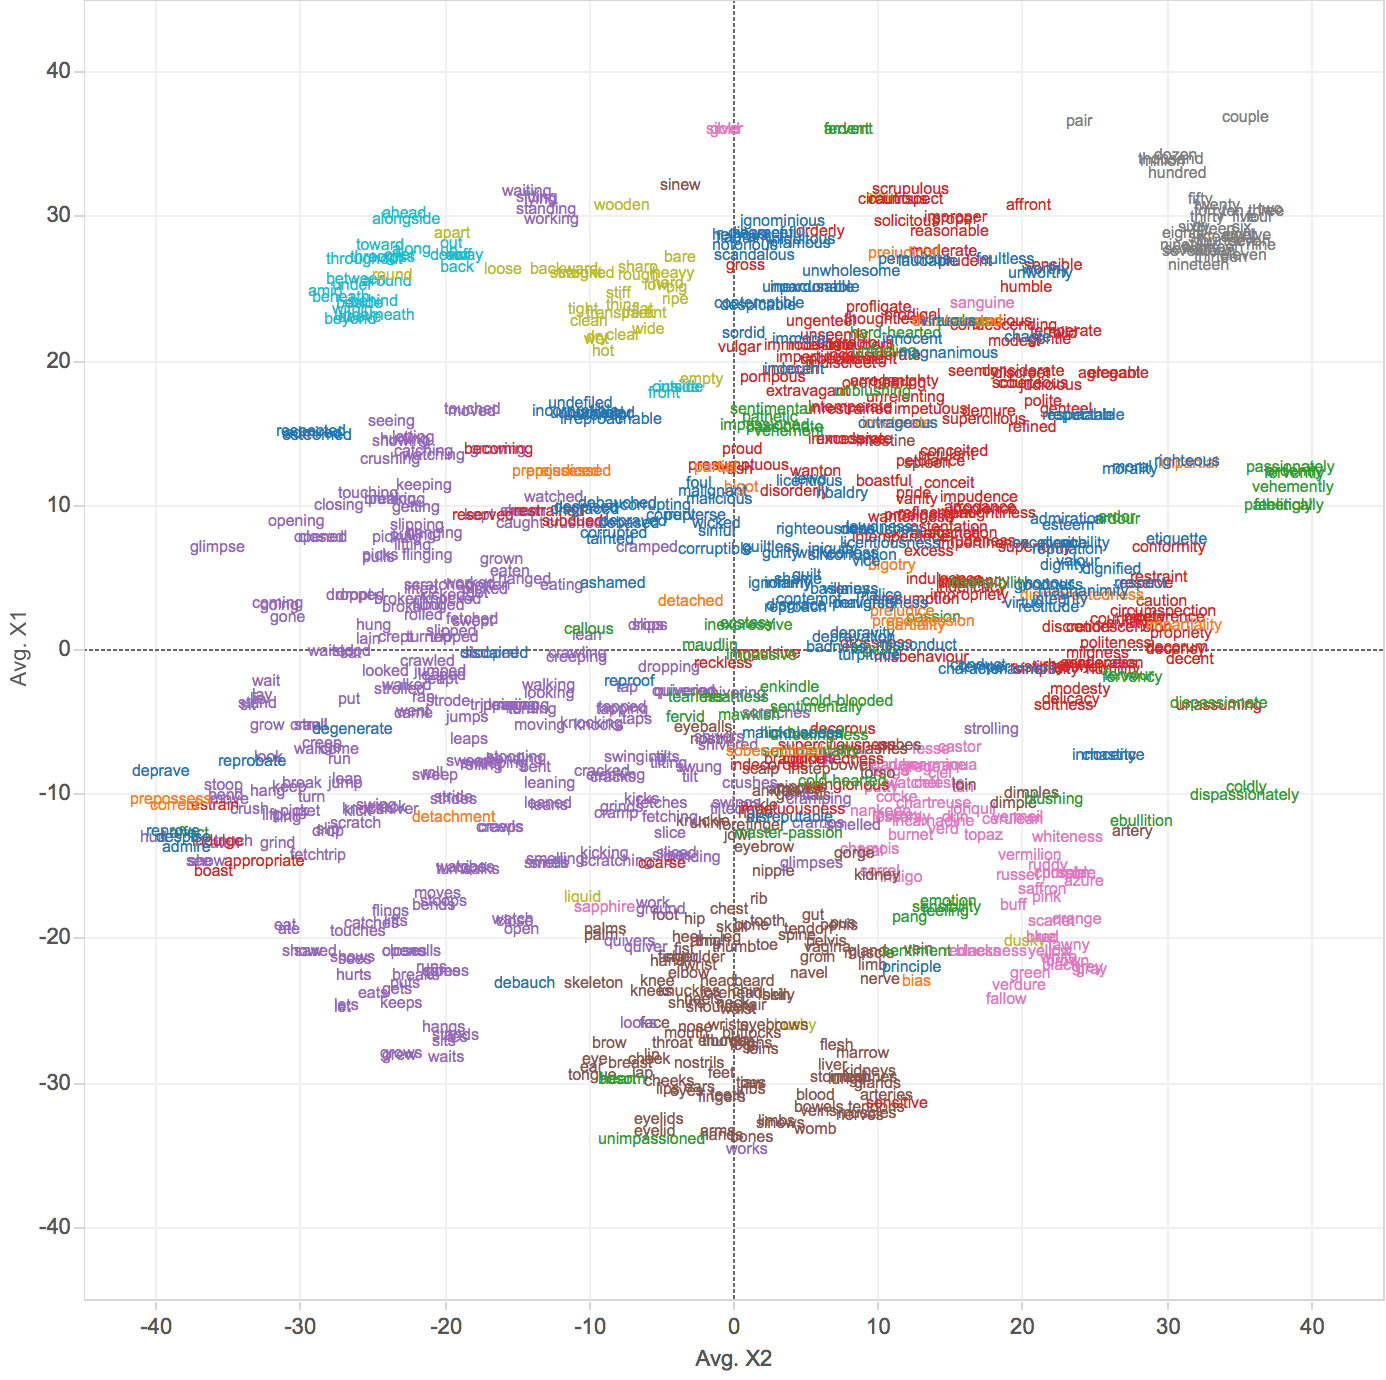
\includegraphics[width=0.7\linewidth]{Fields-to-Vectors-All-words2}
	\caption{Representação semântica lexical?}
	\label{fig:fields-to-vectors-all-words2}
\end{figure}

\end{frame}

%------------------------------------------------


\section{Limitações e problemas}
%------------------------------------------------

\begin{frame}
\begin{itemize}
    \item \Large{Limitações e questões}

\end{itemize}

\end{frame}
%------------------------------------------------


\begin{frame}
\frametitle{Limitações e questões}
\begin{itemize}
\item Sensibilidade ao corpus de treinamento
\item Na prática, é um modelo muito bem sucedido para tarefas de NLP, mas a semantização do modelo é algo complexo.
\item Modelo é treinado a partir de uma quantidade absurda de dados linguísticos. Não possui nenhuma expectativa de ter alguma veracidade neurolinguística.
\item A noção de 'relação semântica' é intuitiva, mas formalmente vaga.
\end{itemize}
\end{frame}


\begin{frame}
\frametitle{ Próximos passos}
\begin{itemize}
\item Investigar um tipo específico de relação semântica: a sinonímia.
\item Analisar o funcionamento da sinonímia nos modelos.
\item Criar classificadores de sinônimos para esse tipo de modelo, usando abordagens matemáticas e/ou linguísticas.
\end{itemize}
\end{frame}

%------------------------------------------------

%------------------------------------------------
\section{Bibliografia}
%------------------------------------------------

\begin{frame}
\frametitle{References}
\footnotesize{
\begin{thebibliography}{} % Beamer does not support BibTeX so references must be inserted manually as below
\bibitem[Mikolov, 2013]{p1} Mikolov et al. (2013). Linguistic regularities in continuous space word representations.\emph{Proceedings of NAACL-HLT 2013}.

\bibitem[Jurafsky, 2018]{p1} Jurafsky, D. \& Martin, J.(2018). Speech and Language Processing.\emph{3rd Edition draft, 2018}.

\bibitem[Bengio, 2003]{p1} Bengio, Y et al (2003). A Neural Probabilistic Language Model.\emph{Journal of Machine Learning Research 3, 2003}.

\bibitem[Manning, 2008]{p1} Manning, C. et al (2008). Introduction to information retrieval.\emph{Cambridge University Press, 2018}.

\bibitem[Widdows, 2004]{p1} Widdows, D. (2004). Geometry and Meaning.\emph{CSLI Publications, 2004}.

\bibitem[Tensorflow]{p1} Tensorflow, Vector Representations of words (2018).\emph{https://www.tensorflow.org/tutorials/representation/word2vec}.

\bibitem[Colyer, 2016]{p1} Colyer, A. The amazing power of word vectors (2016).\emph{https://blog.acolyer.org/2016/04/21/the-amazing-power-of-word-vectors/}.

\bibitem[Deisenroth, 2018]{p1} Deisenroth, M.P. et al (2018). Mathematics for Machine Learning.\emph{Cambridge University Press, 2018}.
\end{thebibliography}
}
\end{frame}

%------------------------------------------------

\begin{frame}
\begin{figure}
	\centering
	
\includegraphics[width=0.7\linewidth]{curse-of-dimensionality}
	\caption{Obrigado!}
	\label{fig:curse-of-dimensionality}
\end{figure}

\end{frame}

%----------------------------------------------------------------------------------------

\end{document}